

\tikzset{every picture/.style={line width=0.75pt}} %set default line width to 0.75pt        

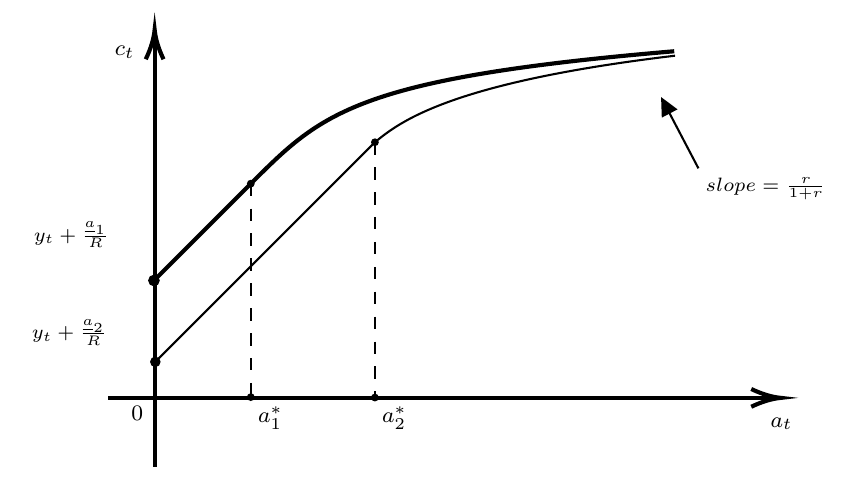
\begin{tikzpicture}[x=0.75pt,y=0.75pt,yscale=-1,xscale=1]
%uncomment if require: \path (0,309); %set diagram left start at 0, and has height of 309

%Straight Lines [id:da8411624928883772] 
\draw [line width=1.5]    (116.33,254) -- (437.33,254) ;
\draw [shift={(440.33,254)}, rotate = 180] [color={rgb, 255:red, 0; green, 0; blue, 0 }  ][line width=1.5]    (14.21,-4.28) .. controls (9.04,-1.82) and (4.3,-0.39) .. (0,0) .. controls (4.3,0.39) and (9.04,1.82) .. (14.21,4.28)   ;
%Straight Lines [id:da5652262602936624] 
\draw [line width=1.5]    (138.67,287.07) -- (138.67,79.64) ;
\draw [shift={(138.67,76.64)}, rotate = 90] [color={rgb, 255:red, 0; green, 0; blue, 0 }  ][line width=1.5]    (14.21,-4.28) .. controls (9.04,-1.82) and (4.3,-0.39) .. (0,0) .. controls (4.3,0.39) and (9.04,1.82) .. (14.21,4.28)   ;
%Curve Lines [id:da6438367824501467] 
\draw [color={rgb, 255:red, 0; green, 0; blue, 0 }  ,draw opacity=1 ][line width=1.5]    (185,150.79) .. controls (219,117) and (235,100) .. (389,87) ;
%Curve Lines [id:da36694400011089146] 
\draw [color={rgb, 255:red, 0; green, 0; blue, 0 }  ,draw opacity=1 ][line width=0.75]    (244.8,130.84) .. controls (257,120.74) and (281.8,101.94) .. (389.4,89.14) ;
%Straight Lines [id:da38094524039195865] 
\draw [color={rgb, 255:red, 0; green, 0; blue, 0 }  ,draw opacity=1 ]   (244.8,130.84) -- (139,236.64) ;
\draw [shift={(139,236.64)}, rotate = 135] [color={rgb, 255:red, 0; green, 0; blue, 0 }  ,draw opacity=1 ][fill={rgb, 255:red, 0; green, 0; blue, 0 }  ,fill opacity=1 ][line width=0.75]      (0, 0) circle [x radius= 2.01, y radius= 2.01]   ;
%Straight Lines [id:da1747827710510499] 
\draw [color={rgb, 255:red, 0; green, 0; blue, 0  }  ,draw opacity=1 ][line width=1.5]    (185,150.79) -- (138.33,197.45) ;
\draw [shift={(138.33,197.45)}, rotate = 135] [color={rgb, 255:red, 0; green, 0; blue, 0 }  ,draw opacity=1 ][fill={rgb, 255:red, 0; green, 0; blue, 0 }  ,fill opacity=1 ][line width=1.5]      (0, 0) circle [x radius= 1.74, y radius= 1.74]   ;
%Straight Lines [id:da6520435098688784] 
\draw [color={rgb, 255:red, 0; green, 0; blue, 0 }  ,draw opacity=1 ][line width=0.75]  [dash pattern={on 4.5pt off 4.5pt}]  (185,150.79) -- (185,253.64) ;
\draw [shift={(185,253.64)}, rotate = 90] [color={rgb, 255:red, 0; green, 0; blue, 0 }  ,draw opacity=1 ][fill={rgb, 255:red, 0; green, 0; blue, 0 }  ,fill opacity=1 ][line width=0.75]      (0, 0) circle [x radius= 1.34, y radius= 1.34]   ;
\draw [shift={(185,150.79)}, rotate = 90] [color={rgb, 255:red, 0; green, 0; blue, 0 }  ,draw opacity=1 ][fill={rgb, 255:red, 0; green, 0; blue, 0 }  ,fill opacity=1 ][line width=0.75]      (0, 0) circle [x radius= 1.34, y radius= 1.34]   ;
%Straight Lines [id:da6381161981070622] 
\draw [color={rgb, 255:red, 0; green, 0; blue, 0 }  ,draw opacity=1 ][line width=0.75]  [dash pattern={on 4.5pt off 4.5pt}]  (244.8,130.84) -- (244.8,253.84) ;
\draw [shift={(244.8,253.84)}, rotate = 90] [color={rgb, 255:red, 0; green, 0; blue, 0 }  ,draw opacity=1 ][fill={rgb, 255:red, 0; green, 0; blue, 0 }  ,fill opacity=1 ][line width=0.75]      (0, 0) circle [x radius= 1.34, y radius= 1.34]   ;
\draw [shift={(244.8,130.84)}, rotate = 90] [color={rgb, 255:red, 0; green, 0; blue, 0 }  ,draw opacity=1 ][fill={rgb, 255:red, 0; green, 0; blue, 0 }  ,fill opacity=1 ][line width=0.75]      (0, 0) circle [x radius= 1.34, y radius= 1.34]   ;
%Straight Lines [id:da42499965052938493] 
\draw [color={rgb, 255:red, 0; green, 0; blue, 0 }  ,draw opacity=1 ]   (400.67,143.42) -- (384.06,111.74) ;
\draw [shift={(382.67,109.08)}, rotate = 62.33] [fill={rgb, 255:red, 0; green, 0; blue, 0 }  ,fill opacity=1 ][line width=0.08]  [draw opacity=0] (8.93,-4.29) -- (0,0) -- (8.93,4.29) -- cycle    ;

% Text Node
\draw (118,83) node [anchor=north west][inner sep=0.75pt]  [font=\footnotesize] [align=left] {$c_{t}$};
% Text Node
\draw (434,262) node [anchor=north west][inner sep=0.75pt]  [font=\footnotesize] [align=left] {$a_{t}$};
% Text Node
\draw (126,256.66) node [anchor=north west][inner sep=0.75pt]  [font=\footnotesize] [align=left] {$0$};
% Text Node
\draw (187,256.64) node [anchor=north west][inner sep=0.75pt]  [font=\footnotesize] [align=left] {$a^{\ast}_{1}$};
% Text Node
\draw (246.8,256.84) node [anchor=north west][inner sep=0.75pt]  [font=\footnotesize] [align=left] {$a^{\ast}_{2}$};
% Text Node
\draw (79,167.66) node [anchor=north west][inner sep=0.75pt]  [font=\scriptsize] [align=left] {$y_{t} +\frac{\underline{a}_{1}}{R}$};
% Text Node
\draw (78,214.66) node [anchor=north west][inner sep=0.75pt]  [font=\scriptsize] [align=left] {$y_{t} +\frac{\underline{a}_{2}}{R}$};
% Text Node
\draw (402.67,146.42) node [anchor=north west][inner sep=0.75pt]  [font=\scriptsize,color={rgb, 255:red, 0; green, 0; blue, 0 }  ,opacity=1 ] [align=left] {$slope=\frac{r}{1+r}$};


\end{tikzpicture}
